\chapter{Polly}
One of the numerous subprojects of the \llvm is Polly\footnote{The name \enquote{Polly} is combination of \enquote{Polyhedral} and \enquote{\llvm}. \cite{PollyGrosser}} which provides plenty of options for automatic optimizations based on the polyhedral model operating on \llvmir.

\section{Geschichte}
Polly was first described in the publication \cite{PollyGrosser}.\draftnote{TODO: More information?}

\section{The pipeline of Polly}
Polly uses the same pipeline as \llvm but it is a plugin for the \opt. Before using Polly the option \texttt{-O3} has to specified while generating \llvmir using the clang frontend.
Afterwards the library of Polly and its additional options have to be loaded by the \opt (\autoref{subsec:optimizer}).
\begin{figure}[h]
    \caption[The pipeline of Polly]{The pipeline of Polly \cite{PollyPresentation}}
    \centering
    \begin{tikzpicture}
        \coordinate(clang);
        \node(opt)[llvmIrNode, right=of clang]{\ac{LLVM} Optimizer};
        \node(polly)[llvmIrNode, below=of opt]{\ac{LLVM} Polly};
        \coordinate[right=of opt](generator);
        \path[llvmIrPath] (clang) to (opt);
        \path[llvmIrPath, bend right] (opt.south west) to node[auto, swap]{SCoP Detection} (polly);
        \path[llvmIrPath, bend right] (polly) to node[auto, swap]{Code Generation} (opt.south east);
        \path[llvmIrPath] (opt) to (generator);
        \path[llvmIrPath] (polly) edge[loop below] ();
        \path[llvmIrPath] (opt) edge[loop above] node[auto]{Pass} ();
    \end{tikzpicture}
\end{figure}\\
There are two essential terms for understanding Polly. On the one hand it is \enquote{region} on the other hand it is \enquote{\scop}.
\subsection{Definition region}\label{subsec:definitionRegion}
In \cite[chapter 9.7.1, p.~672]{Drachenbuch} a region is defined as:
\begin{comment}
    Seite 672, Chapter 9. Machine-independent optimizations, 9.7.1 Regions
\end{comment}
\begin{quote}
    Formally, a region of a flow graph is a collection of nodes N and edges E such that:
    \begin{enumerate}
        \item There is a header h in N that dominates all the nodes in N.
        \item If some node m can reach a node n in N without going through h, then m is also in N.
        \item E is the set of all the control flow edges between nodes \(n_1\) and \(n_2\) in N, except (possibly) for some that enter h.
    \end{enumerate}
\end{quote}
In \autoref{fig:exampleRegion} the regions of \autoref{lst:matmulll} are shown.
\begin{figure}[!ht]
    \centering
    \caption{The regions of \autoref{lst:matmulll}}
    \label{fig:exampleRegion}
    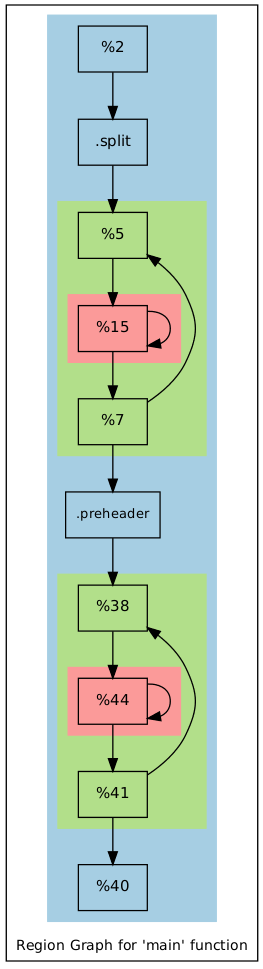
\includegraphics[width=\textwidth]{gfx/matmulRegions.png}
\end{figure}\\
For visualizing the regions of \autoref{lst:matmulcpp} a dot file is generated using the option \texttt{-view-regions-only}:
\begin{enumerate}
    \item Translate the C++ sourcecode into \llvmir (\autoref{lst:matmulll})\\
        \texttt{clang -S -emit-llvm matmul.cpp -o matmul.ll}
    \item Generate the regiontree\\
        \texttt{opt -view-regions-only matmul.ll}
\end{enumerate}
\subsection{Definition SCoP}\label{subsec:definitionScop}
\begin{comment}
    Copy\&pasted from polly/lib/Analysis/ScopDetection.cpp

    A static control part (Scop) is a subgraph of the control flow graph (CFG)
    that only has statically known control flow and can therefore be described
    within the polyhedral model.

    Every Scop fulfills these restrictions:
    * It is a single entry single exit region
    * Only affine linear bounds in the loops

    Every natural loop in a Scop must have a number of loop iterations that can
    be described as an affine linear function in surrounding loop iterators or
    parameters. (A parameter is a scalar that does not change its value during
    execution of the Scop).
    * Only comparisons of affine linear expressions in conditions
    * All loops and conditions perfectly nested

    The control flow needs to be structured such that it could be written using
    just 'for' and 'if' statements, without the need for any 'goto', 'break' or
    'continue'.

    * Side effect free functions call

    Function calls and intrinsics that do not have side effects (readnone)
    or memory intrinsics (memset, memcpy, memmove) are allowed.
\end{comment}
A \scop is a certain type of region on which optimizations in top of the polyhedral model can be performed.
More precisly it is a subgraph of the \cfg that only has statically known control flow and can therefore be described within the polyhedral model.
Every \scop fulfills these restrictions according to ScopDetection:
\begin{itemize}
    \item It is a single entry single exit region (\autoref{subsec:definitionRegion}).
    \item Only affine linear bounds in the loops.\\
        Every natural loop in a \scop must have a number of loop iterations that can be described as an affine linear function in surrounding loop iterators or parameters. (A parameter is a scalar that does not change its value during execution of the Scop).
    \item Only comparisons of affine linear expressions in conditions.
    \item All loops and conditions perfectly nested.\\
        The control flow needs to be structured such that it could be written using just \mintinline{c++}{for} and \mintinline{c++}{if} statements, without the need for any \mintinline{c++}{goto}, \mintinline{c++}{break} or \mintinline{c++}{continue}.
    \item Side effect free functions call.\\
        Function calls and intrinsics that do not have side effects (readnone) or \enquote{memory intrinsics (\mintinline{c++}{memset, memcpy, memmove}) are allowed}.
\end{itemize}
The visualization of the \scops of \autoref{lst:matmulcpp} is shown in \autoref{fig:exampleScop}.
\begin{figure}[!ht]
    \centering
    \caption{The SCoPs of \autoref{lst:matmulpreoptll}}
    \label{fig:exampleScop}
    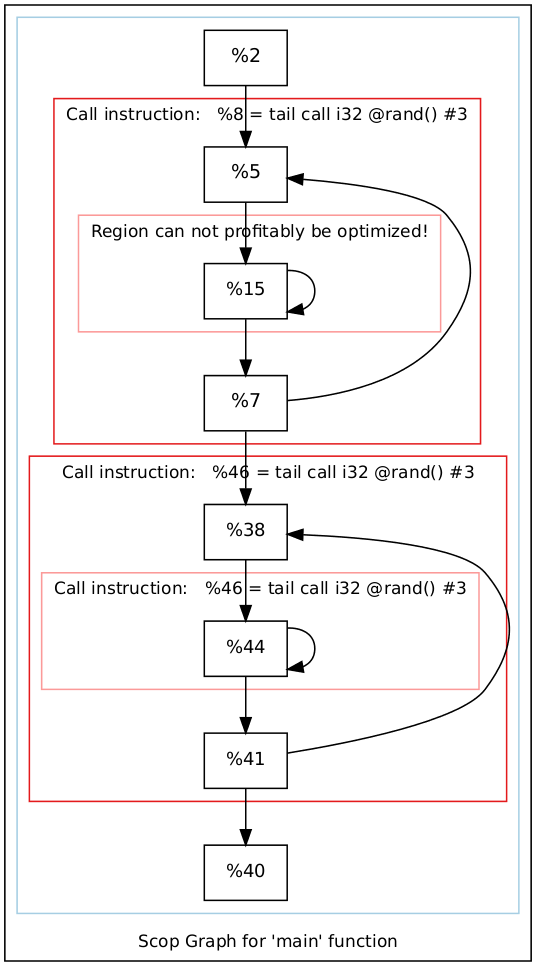
\includegraphics[height=15cm]{gfx/matmulScops.png}
\end{figure}
The dot file is generated by the option \texttt{-view-scops-only}:
\begin{enumerate}
    \item Translate the C++ sourcecode into \llvmir (\autoref{lst:matmulllO3})\\
        \texttt{clang -S -emit-llvm -O3 matmul.cpp -o matmul.ll}
    \item Prepare the \llvmir for Polly (\autoref{lst:matmulpreoptll})\\
        \texttt{opt -S -load LLVMPolly.so -polly-canonicalize matmul.ll > matmul.preopt.ll}
    \item Generate the \scop tree\\
        \texttt{opt -load LLVMPolly.so -disable-output -view-scops-only matmul.preopt.ll}
\end{enumerate}

\section{SCoPDetection}
Before any operation can be done by Polly, Polly has to identify regions having sufficient criteria for being a \scop under certain assumptions.
When choosing candidates for \scops the following assumptions are taken.
\begin{description}
    \item[Aliasing]
    \item[Inbounds]
    \item[Wrapping]
    \item[unasigned]
    \item[complexity]
    \item[unprofitable]
    \item[errorBlock]
    \item[infiniteLoop]
    \item[invariantLoad]
    \item[delinearization]
\end{description}
\begin{comment}
    Copy\&pasted from ScopInfo.cpp

    STATISTIC(AssumptionsAliasing, "Number of aliasing assumptions taken.");
    STATISTIC(AssumptionsInbounds, "Number of inbounds assumptions taken.");
    STATISTIC(AssumptionsWrapping, "Number of wrapping assumptions taken.");
    STATISTIC(AssumptionsUnsigned, "Number of unsigned assumptions taken.");
    STATISTIC(AssumptionsComplexity, "Number of too complex SCoPs.");
    STATISTIC(AssumptionsUnprofitable, "Number of unprofitable SCoPs.");
    STATISTIC(AssumptionsErrorBlock, "Number of error block assumptions taken.");
    STATISTIC(AssumptionsInfiniteLoop, "Number of bounded loop assumptions taken.");
    STATISTIC(AssumptionsInvariantLoad,
              "Number of invariant loads assumptions taken.");
    STATISTIC(AssumptionsDelinearization,
              "Number of delinearization assumptions taken.");
\end{comment}
Afterwards these candidates are again analysed for determing whether these are valid \scops.
